\documentclass[11pt,a4paper]{scrreprt}
\usepackage[ngerman]{babel}
\usepackage{fullpage}
\usepackage[utf8]{inputenc}
\usepackage{graphicx} 
\usepackage{footmisc}

\usepackage{placeins}
\usepackage{epstopdf}
\usepackage{hyperref}


\usepackage{listings}

\setlength{\parindent}{0.0in}
\setlength{\parskip}{0.1in}

\renewcommand*{\chapterheadstartvskip}{\vspace*{-25pt}}	

\begin{document}

\title{Asymmetrische Kryptografie in Java}
\subtitle{Sichere verteilte Anwendungen mit Java\\
		%	Lehrstuhl Betriebssysteme und Verteilte Systeme\\
		%	Institut für Informatik\\
		%	Universität Potsdam
		}
\author{Alexander H. W. Lindemann}
\date{17. Januar 2014}
\maketitle

\tableofcontents

\chapter{Theoretische Grundlagen}
\section{Ziele}
Asymmetrische Kryptografie und Kryptografie im Allgemeinen haben zum Ziel, Nachrichten (Daten, Texte, etc.) so zu manipulieren, dass sie nur vom jeweiligen Empfänger gelesen werden können. Hierbei werden komplexe mathematische Probleme als Grundlage gewählt, um das unberechtigte Lesen der Nachricht zu verhindern.

\section{Asymmetrische Kryptografie}
Im Gegensatz zur symmetrischen Kryptografie, werden bei der asymmetrischen Kryptografie 2 Schlüssel, also ein Schlüsselpaar, benutzt. Einer der beiden wird als öffentlicher Schlüssel, der andere als privater Schlüssel bezeichnet. Mit dem öffentlichen Schlüssel werden die Nachrichten verschlüsselt und mit dem privaten Schlüssel wieder entschlüsselt. Daraus folgt, das der private Schlüssel nur dem Empfänger bekannt sein sollte. 

\section{SYSTEM}
\begin{figure}[hbtp]
\caption{Kryptosysteme nach \cite{Eckert13}}
\centering
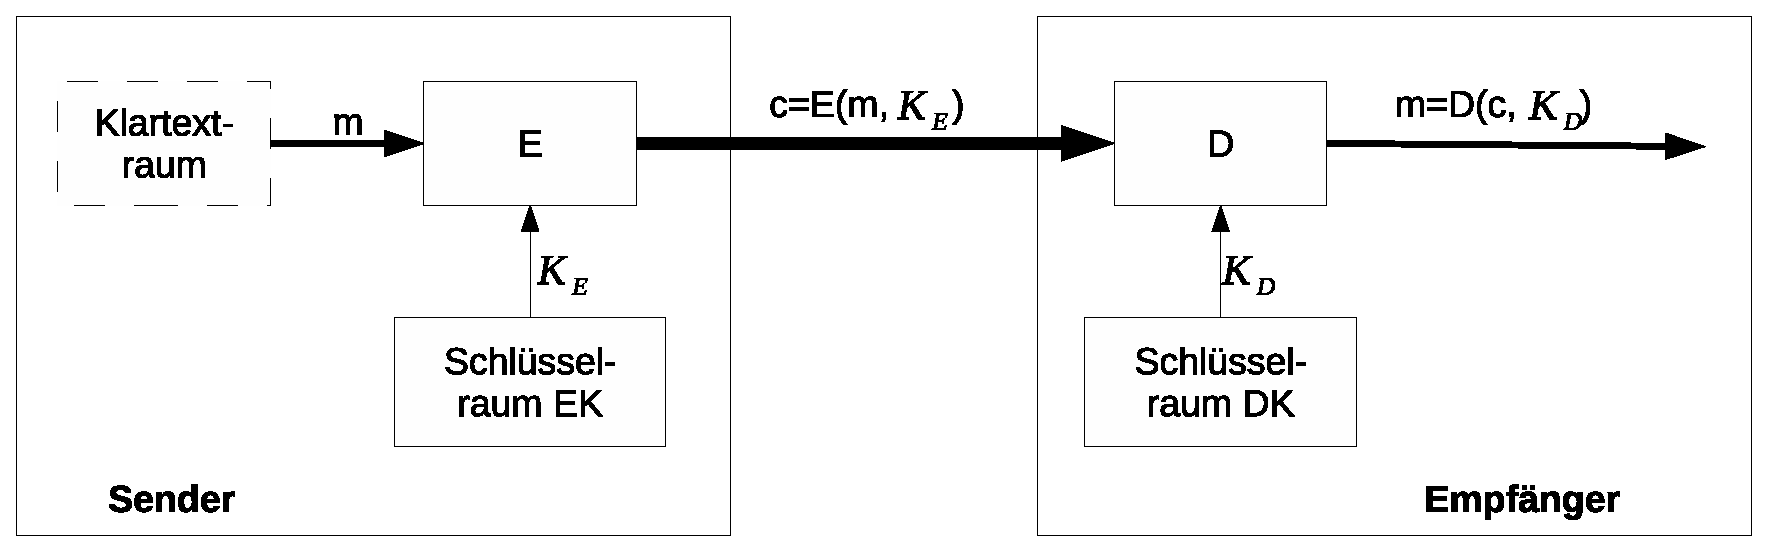
\includegraphics[width=\textwidth]{async.eps}
\begin{minipage}[t]{0.45\linewidth}
\centering
\begin{itemize}
\item Tupel = ($M,C,EK,DK,E,D$)
\item 2 endliche Alphabete ($A_1,A_2$)
\item Klartext ($M \subseteq A^*_1\backslash\emptyset$)
\item Kryptotext ($C \subseteq A^*_2\backslash\emptyset$)
\item Verschlüsselungsschlüsselraum ($EK\backslash\emptyset$)
\item Es gilt:
\\ $\forall m\in M : D(E(m,K_E),K_D) = m$
\end{itemize}
\end{minipage}
\begin{minipage}[t]{0.45\linewidth}
\begin{itemize}
\item Entschlüsselungsschlüsselraum\\
($DK/\emptyset \\mit~ f:EK \rightarrow DK \\und~ f(K_E)=K_D)$
\item Verschlüsselungsverfahren ($E :~ M x EK \rightarrow C$)
\item Entschlüsselungsverfahren ($D :~ C x DK \rightarrow M$)
\end{itemize}
\end{minipage}
\label{KryptoSys}
\end{figure}

Ein Kryptosystem besteht, laut \cite{Eckert13} aus den in Abbildung \ref{KryptoSys} dargestellten Komponenten. 

\section{Einwegfunktionen}
Eine Einwegfunktion ist eine Funktion, welche nach komplexitätstheoretischen Maßstäben leicht zu berechnen, aber schwer umzukehren ist. Meist werden Funktionen so bezeichnet welche sich nicht in angemessener Zeit umkehren lassen. Diese Eigenschaft macht sie ideal zur Verwendung in Kryptografischen Algorithmen, da so sichergestellt ist das die Nachricht nicht unberechtigt entschlüsselt wird. Leider verhindern solche Funktionen das Entschlüsseln vollständig, weshalb eine andere Kategorie von Funktionen zum Einsatz kommt, die so genannten \textbf{Einwegfunktionen mit Falltür}.

Einwegfunktionen mit Falltür haben den Vorteil, dass mit gewissem Zusatzwissen die Umkehrung leicht zu berechnen ist. Dieses Zusatzwissen wird in der asymmetrischen Kryptografie im privaten Schlüssel gespeichert, was garantiert das nur der richtige Empfänger die Nachricht entschlüsseln kann.


\section{Beispiel RSA}
Ein Beispiel für ein asymmetrisches Verschlüsselungsverfahren ist der \textit{RSA} Algorithmus. Dieser basiert auf einer Einwegpermutation mit Falltür. 

\subsection{Schlüsselgenerierung}
Ein Schlüsselpaar besteht bei RSA aus folgenden Komponenten:
\begin{itemize}
\item Öffentlicher Schlüssel - $(e,N)$
\item Privater Schlüssel - $(d,N)$
\end{itemize}

Wobei $N$ das \textit{RSA-Modul} genannt wird, $e$ der Verschlüsselungsexponent und $d$ der Entschlüsselungsexponent. Diese Zahlen werden nach folgendem Verfahren bestimmt:
\begin{enumerate}
\item Man wähle 2 zufällige und voneinander (stochastisch) unabhängige Primzahlen $p\neq q$
\item Nun wird $N = p \cdot q$ berechnet
\item Danach muss $\varphi(N) = (p-1)\cdot(q-1)$ bestimmt werden
\item Man wähle nun eine Zahl zu $\varphi(N)$ teilerfremde Zahl $e$ für die gilt: $1<e<\varphi(N)$
\item $d$ wird nun als multiplikativ Inverses zu $e$ bzgl. $\varphi(N)$ bestimmt.
\\($e \cdot d \equiv 1 ~mod~ \varphi(N)$)
\end{enumerate} 
Nach der Generierung der Schlüsseldaten $d$ und $e$ können und sollten $\varphi(N)$, $p$ und $q$ gelöscht werden, um die unbefugte Rekonstruktion des Privaten Schlüssels zu verhindern. 

\subsection{Ver- und Entschlüsselung}
Um mithilfe eines Schlüsselpaares Nachrichten zu ver- und entschlüsseln kommen folgende Formeln zum Einsatz:
\begin{itemize}
\item $c \equiv m^e ~mod~  N$
\item $m \equiv c^d ~mod~  N$
\end{itemize}
Wobei $m$ die Nachricht und $c$ den aus der Nachricht abgeleiteten chiffrierten Text darstellt.

Da die Operationen auch invers durchführbar sind, man also mit dem privaten Schlüssel Nachrichten chiffrieren kann welche dann durch den öffentlichen Schlüssel dechiffriert werden können, kann man mit diesem Verfahren eine so genannte digitale Signatur durchführen. Hierbei wird meist auf den Hash einer Nachricht der eigene privaten Schlüssel angewendet und dieser dann an die Nachricht angehängt. Der Empfänger kann nun eindeutig bestimmen ob die Nachricht während des Transports verändert wurde (der Hash würde dann nicht stimmen) und ob die Nachricht wirklich vom angegebenen Versender verfasst wurde (der öffentliche Schlüssel muss zur Signatur passen).

\section{Hybride Kryptografie}
Hybride Kryptografie ist eine Kombination aus symmetrischer und asymmetrischer Kryptografie. Hierbei wird eine Nachricht erst symmetrisch verschlüsselt und der symmetrische Sitzungsschlüssel dann über einen asymmetrisch gesicherten Kanal ausgehandelt oder an die Nachricht angehängt. Der Empfänger kann den Sitzungsschlüssel dann entschlüsseln und so die Nachricht lesen.

Dieses Verfahren hat den Vorteil das die komplexen Berechnungsschritte, welche für asymmetrische Verfahren notwendig sind, nur auf den Sitzungsschlüssel angewendet werden. 

Ein weiterer Vorteil besteht darin, dass  eine gebrochene Nachricht nicht die Kompromittierung der gesamten Kommunikation bedeutet sondern nur die Offenlegung der jeweiligen Sitzung.


\chapter{Kryptografie mit Java}
\section{Java Cryptography Architecture}

\section{Zufallszahlen}
Ein wichtiger Punkt bei der Erzeugung von Schlüsseln und der anschließenden Durchführung von Kryptooperationen ist die Bereitstellung von geeigneten Zufallszahlen, da sonst das Erraten des Schlüssels oder das zurückrechnen von Kryyptooperationen zu einfach werden könnte.

Die JCA bietet hier die Möglichkeit über die Klasse \textit{java.security.SecureRandom} eigene Zufallszahlengeneratoren per Kryptoprovider bereitzustellen. Weiterhin wird mit der SunJCE-Implementierung ein eigener Generator angeboten. Hierbei müssen einigen Richtlinien für Zufallszahlengeneratoren beachtet werden, unter anderem die \textit{FIPS 140-2}-Richtlinie\footnote{\url{http://csrc.nist.gov/publications/fips/fips140-2/fips1402.pdf}} und der \textit{RFC 1750}\footnote{\url{http://www.ietf.org/rfc/rfc1750.txt}}. Weiterhin ist zu beachten das der Seed mit dem die Generatoren initialisiert werden zufällig sein sollte.

\section{Schlüsselgenerierung}

\begin{figure}[hbtp]
\caption{Codebeispiel KeyPairGenerator}
\begin{lstlisting}[frame=shadowbox]
 KeyPairGenerator keyGen = 
 	KeyPairGenerator.getInstance( "RSA" );
 keyGen.initialize( int keysize );
 KeyPair keys = keyGen.generateKeyPair();
\end{lstlisting}
(KeyGenerator ist analog zu benutzen)
\label{KeyPairGen}
\end{figure}

Schlüssel werden unter Java mit den Klassen \textit{java.security.KeyPairGenerator} (Schlüsselpaar) bzw. \textit{javax.crypto.KeyGenerator} (Symmetrischer Schlüssel) erzeugt. Diese können über die in Abbildung \ref{KeyPairGen} dargestellten Codezeilen instanziiert und genutzt werden. Hierbei ist es möglich den gewünschten Algorithmus, die Schlüssellänge und den Zufallszahlengenerator als Parameter zu übergeben.

\section{Schlüsselspeicherung}
Schlüssel werden in Java mithilfe der Klasse \textit{java.security.KeyStore} gespeichert, jedoch ist es auch möglich die Schlüsselpaare als \textit{java.security.KeyPair} in serialisierter Form auf die Festplatte zu speichern. Dabei werden jedoch die Schlüsseldaten nicht gegen unbefugtes öffnen gesichert, deshalb ist in produktiven Umgebungen immer eine Speicherung via Keystore vorzuziehen. Der Keystore erlaubt die Speicherung einer belieben Anzahl von Schlüsseln und Zertifikaten, sowie die Sicherung dieser mithilfe unterschiedlicher Passwörter, sowie weiteren Mechanismen.

Eine weitere Methode zur Schlüsselspeicherung wird über das Interface \textit{
java.security.Key} bereitgestellt. Die Methode \textit{getEncoded()} liefert die Repräsentation des Schlüssels in einem, per \textit{getFormat} abzurufenden, Format, Beispielsweise \textit{x.509} oder \textit{PKCS \#8}.

\section{Schlüsseleinigung}

\begin{figure}[hbtp]
\caption{Codebeispiel KeyAgreement}
\begin{lstlisting}[frame=shadowbox]
 KeyAgreement aKeyAgree =
  	KeyAgreement.getInstance("DH", "JCE");
 KeyAgreement bKeyAgree = 
  	KeyAgreement.getInstance("DH", "JCE");
   
 KeyPair aPair = keyGen.generateKeyPair();
 KeyPair bPair = keyGen.generateKeyPair();
 
 aKeyAgree.init(aPair.getPrivate());
 bKeyAgree.init(bPair.getPrivate());
 
 aKeyAgree.doPhase(bPair.getPublic(), true);
 bKeyAgree.doPhase(aPair.getPublic(), true);

 SecretKey aSecret =
   	aKeyAgree.generateSecret("AES");
 SecretKey bSecret =
   bKeyAgree.generateSecret("AES");
\end{lstlisting}
\label{KeyAgree}
\end{figure}

Falls während eines Verbindungsaufbaus eine Schlüsseleinigung notwendig sein sollte, so wird dies durch die Klasse \textit{javax.crypto.KeyAgreement} ermöglicht. Hierbei wird meist\footnote{SunJCE und Bouncy Castle unterstützen hier nur Varianten des Diffie–Hellman Algorithmus} der Diffie–Hellman Algortihmus benutzt. In der Abbildung \ref{KeyAgree} wird gezeigt wie diese Klasse zu verwenden ist. Hierbei ist zu beachten, das nach der Intitialisierung mit dem eigenen privaten Schlüssel, die Methode \textit{doPhase()} mit den öffentlichen Schlüsseln der Gesprächspartner ausgeführt wird. Beim Aufruf der Methode mit dem Schlüssel des letzten Partners ist der zweite Parameter auf "`true"' zu setzen, um dem System den Abschluss der Operation zu signalisieren. Abschließend kann dann mit der Methode \textit{generateSecret()} ein symmetrischer Sitzungsschlüssel erzeugt werden.

\section{Ver- und Entschlüsselung}


\begin{figure}[hbtp]
\caption{Codebeispiel KeyAgreement}
\begin{lstlisting}[frame=shadowbox]
 Cipher cipher = 
 	Cipher.getInstance( "RSA", "BC" );
 cipher.init( Cipher.ENCRYPT_MODE, publicKey );
 cipher.update( message );
 byte[]crypt = cipher.doFinal();
\end{lstlisting}
\label{encrypt}
\end{figure}


\nocite{Eckert13}
\nocite{Engelbrecht04}
\bibliography{literatur-Java-Security}{}
\bibliographystyle{apalike}
\end{document}



\end{document}